\subsection{GeoGebra: Uvod}

\subsubsection{Kaj je Geogebra?}

\href{https://www.geogebra.org/}{Geogebra} je brezplačno dinamično matematično orodje, ki omogoča raziskovanje in vizualizacijo različnih matematičnih konceptov.

Trenuto, Geogebra je popoln paket za učenje in poučevanje matematike. Ponuja različne aplikacije, ki pokrivajo področja, kot so geometrija, algebra, statistika in kalkulus.
Vse te aplikacije je mogoče namestiti lokalno ali dostopati do njih prek spleta:

\begin{itemize}
\item \href{https://www.geogebra.org/scientific}{Scientific Calculator}: Za izračune z ulomki, statistiko in osnovnimi matematičnimi funkcijami.
\item \href{https://www.geogebra.org/graphing}{Graphing Calculator}: Za vizualizacijo enačb in funkcij z interaktivnimi grafikoni.
\item \href{https://www.geogebra.org/geometry}{Geometry}: Za dinamične geometrijske koncepte in konstrukcije v ravnini.
\item \href{https://www.geogebra.org/3d}{3D Calculator}: Za raziskovanje tridimenzionalnih oblik in površin.
\item \href{https://www.geogebra.org/cas}{CAS Calculator}: Za simbolne izračune in reševanje enačb.
\item \href{https://www.geogebra.org/calculator}{Calculator suit}: Kombinacija različnih orodij za širok spekter matematičnih nalog. Idealna za učence in študente.
\item \href{https://www.geogebra.org/classic}{Geogebra Classic}: Vse-v-enem aplikacija, ki združuje vse zgoraj omenjene funkcije. Idealna za avtorije učnih gradiv.
\end{itemize}

Različne možnosti, ki jih ponuja vsako od orodij, so navedene v Table~\ref{tab_geogebra-apps}.

\begin{table}
\centering
\caption[]{Primerjava različnih aplikacij Geogebra}
\label{tab_geogebra-apps}
\begin{tabular}{p{\dimexpr 0.125\linewidth-2\tabcolsep}p{\dimexpr 0.125\linewidth-2\tabcolsep}p{\dimexpr 0.125\linewidth-2\tabcolsep}p{\dimexpr 0.125\linewidth-2\tabcolsep}p{\dimexpr 0.125\linewidth-2\tabcolsep}p{\dimexpr 0.125\linewidth-2\tabcolsep}p{\dimexpr 0.125\linewidth-2\tabcolsep}p{\dimexpr 0.125\linewidth-2\tabcolsep}}
\toprule
aplikacije / funkcije & Scientific & Graphing & Geometry & 3D & CAS & Suit & Classic \\
\hline
Numerični izračuni & x & x & x & x & x & x & x \\
Funkcije & x & x & x & x & x & x & x \\
Operacije z ulomki & x & x & x & x & x & x & x \\
Grafično prikazovanje &  & x & x & x & x & x & x \\
Drsniki &  & x & x & x & x & x & x \\
Vektorji in matrike &  & x & x & x & x & x & x \\
Tabele &  & x &  &  & x & x & x \\
Geometrijske konstrukcije &  &  & x & x & x & x & x \\
3D prikazovanje &  &  &  & x &  & x & x \\
Verjetnost in statistika &  &  &  &  &  & x & x \\
Odvodi in integrali &  &  &  & x & x & x & x \\
Reševanje enačb &  &  &  & x & x & x & x \\
Simbolni izračuni &  &  &  & x & x & x & x \\
Spreadsheets &  &  &  &  &  &  & x \\
\bottomrule
\end{tabular}
\end{table}

Mi bomo v nadaljevanju uporabljali predvsem \href{https://www.geogebra.org/classic}{Geogebra Classic}, saj omogoča uporabo vseh orodij na enem mestu.

\subsubsection{Kako začnemo z Geogebro?}

Geogebra lahko uporabimo na dva načina: prek spletnega brskalnika ali z namestitvijo aplikacije na računalnik (ali telefon/tablet).

V vsakem primeru bomo uporabili račun Geogebra, ki nam omogoča shranjevanje naših delovnih zvezkov v oblak in dostop do njih od kjerkoli.

Zdaj imate dve možnosti za začetek uporabe Geogebre:

\begin{enumerate}
\item \textbf{Uporaba spletnega brskalnika}:

\begin{itemize}
\item Obiščite \href{https://www.geogebra.org/classic}{Geogebra Classic}.
\item Kliknite na gumn  
\includegraphics[width=0.0275\linewidth]{files/16px-Menu-button-ope-f5b0cc09aa629bb7475641338f148b1b.png}

 \textit{Menu} v zgornjem levem kotu.
\item Prijavite se s svojim računom z klikom na  
\includegraphics[width=0.0275\linewidth]{files/16px-Menu-signin-720b9ea9464a31ca1f9e7d8d070c2f8e.png}

 \textit{Sign in}.
\end{itemize}


\item \textbf{Namestitev aplikacije}:

\begin{itemize}
\item Prenesite aplikacijo Geogebra Classic za vaš operacijski sistem z \href{https://geogebra.github.io/docs/reference/en/GeoGebra\_Installation/\#\_geogebra\_classic\_6}{uradne strani za prenos}.
\item Namestite aplikacijo in jo odprite.
\item Prijavite se s svojim računom z klikom na gumb 
\includegraphics[width=0.0275\linewidth]{files/16px-Menu-button-ope-f5b0cc09aa629bb7475641338f148b1b.png}

 \textit{Menu}  v zgornjem levem kotu in nato na 
\includegraphics[width=0.0275\linewidth]{files/16px-Menu-signin-720b9ea9464a31ca1f9e7d8d070c2f8e.png}

 \textit{Sign in} .
\end{itemize}
\end{enumerate}

Ko odprete Geogebro in se prijavite, boste videli glavno delovno okolje. Privzeto je prikazi 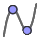
\includegraphics[width=0.0275\linewidth]{files/40px-Menu_view_algeb-122c1ab0ec365e77e9eae26ff7041249.png}

\textit{Graf} (ang. 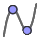
\includegraphics[width=0.0275\linewidth]{files/40px-Menu_view_algeb-122c1ab0ec365e77e9eae26ff7041249.png}

\textit{Graphing perspective}), ki omogoča risanje funkcij in geometrijskih objektov. Lahko jo vidite tudi spodaj:

\begin{framed}
\textbf{Opomba.}\\
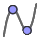
\includegraphics[width=0.0275\linewidth]{files/40px-Menu_view_algeb-122c1ab0ec365e77e9eae26ff7041249.png}

\textit{Graphing perspective} je eden izmed več prikazi, ki jih ponuja Geogebra. Vsaka aplikacija Geogebre je sestavljena iz različnih prikazov, tako da lahko ustvarimo gradiva za različne aplikacije.
Različne prikaze lahko izberemo s klikom na gumb 
\includegraphics[width=0.0275\linewidth]{files/16px-Menu-button-ope-f5b0cc09aa629bb7475641338f148b1b.png}

 \textit{Menu} v zgornjem levem kotu in nato izbiro možnosti 
\includegraphics[width=0.0275\linewidth]{files/16px-Menu-perspectiv-ce02b8b20d416cda63cc58e40cc62dbc.png}

 \textit{Perspectives}.
\end{framed}

Vsak prikaz ponuja različne \textit{poglede} (ang, \textit{views}).
Lahko jih dodamo ali odstranimo glede na naše potrebe s klikom na gumb 
\includegraphics[width=0.0275\linewidth]{files/16px-Menu-button-ope-f5b0cc09aa629bb7475641338f148b1b.png}

 \textit{Menu} v zgornjem levem kotu in nato izbiro možnosti 
\includegraphics[width=0.0275\linewidth]{files/16px-Menu-view.svg-f949496793bee1afbf5580c9151ff29f.png}

 \textit{View}.
Različni pogledi vključujejo:

\begin{itemize}
\item 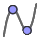
\includegraphics[width=0.0275\linewidth]{files/40px-Menu_view_algeb-122c1ab0ec365e77e9eae26ff7041249.png}

 \textit{Algebrsko okno} (ang. 
\includegraphics[width=0.7\linewidth]{files/16px-Menu_view_algeb-f43b4e7001b948efd7156019d70162e5.png}

\textit{Algebra}).
\item 
\includegraphics[width=0.7\linewidth]{files/16px-Menu_view_cas.s-ac920cb977e8fa51fa4cc9b2de0f21dc.png}

 \textit{Simbolno računanje} (ang. 
\includegraphics[width=0.7\linewidth]{files/16px-Menu_view_cas.s-ac920cb977e8fa51fa4cc9b2de0f21dc.png}

\textit{CAS}).
\item 
\includegraphics[width=0.7\linewidth]{files/16px-Menu_view_graph-07f951165e69080135ae4e0c7469a7db.png}

 \textit{Risalna površina} (ang. 
\includegraphics[width=0.7\linewidth]{files/16px-Menu_view_graph-07f951165e69080135ae4e0c7469a7db.png}

\textit{Graphics}).
\item 
\includegraphics[width=0.7\linewidth]{files/16px-Menu_view_graph-07f951165e69080135ae4e0c7469a7db.png}

 \textit{Grafika 2} (ang. 
\includegraphics[width=0.7\linewidth]{files/16px-Menu_view_graph-2e4bf4b6093ffe88df8ecbb808ff2af0.png}

\textit{Graphics 2}).
\item 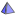
\includegraphics[width=0.7\linewidth]{files/16px-Perspectives_al-4b30a8dd240c5689614b0c4160650a7f.png}

 \textit{3d grafika} (ang. 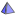
\includegraphics[width=0.7\linewidth]{files/16px-Perspectives_al-4b30a8dd240c5689614b0c4160650a7f.png}

\textit{3D Graphics}).
\item 
\includegraphics[width=0.7\linewidth]{files/16px-Menu_view_sprea-accffca900ee2847b6d4e16428ea9434.png}

 \textit{Preglednica} (ang. 
\includegraphics[width=0.7\linewidth]{files/16px-Menu_view_sprea-accffca900ee2847b6d4e16428ea9434.png}

\textit{Spreadsheet}).
\item 
\includegraphics[width=0.7\linewidth]{files/16px-Menu_view_proba-42fa17d822cb9c58be706d74d5141054.png}

 \textit{Računanje verjetnosti} (ang. 
\includegraphics[width=0.7\linewidth]{files/16px-Menu_view_proba-42fa17d822cb9c58be706d74d5141054.png}

\textit{Probability Calculator}).
\end{itemize}

Drugi vnosi nad gumbom 
\includegraphics[width=0.0275\linewidth]{files/16px-Menu-button-ope-f5b0cc09aa629bb7475641338f148b1b.png}

 \textit{Menu} omogočajo dostop do različnih orodij in nastavitev Geogebre, kot so:

\begin{itemize}
\item 
\includegraphics[width=0.0275\linewidth]{files/16px-Menu-file.svg-b74615e1101cba241695021ac4f1343d.png}

 \textit{Datoteka} (ang. 
\includegraphics[width=0.0275\linewidth]{files/16px-Menu-file.svg-b74615e1101cba241695021ac4f1343d.png}

\textit{File}): Ustvarjanje, odpiranje, shranjevanje in izvoz datotek.
\item 
\includegraphics[width=0.0275\linewidth]{files/16px-Menu-edit.svg-db315b9e8b33fcb7c2a004c62d0b43a2.png}

 \textit{Uredi} (ang. 
\includegraphics[width=0.0275\linewidth]{files/16px-Menu-edit.svg-db315b9e8b33fcb7c2a004c62d0b43a2.png}

\textit{Edit}): Razveljavi, ponovi, kopiraj, prilepi in druge osnovne funkcije urejanja.
\item 
\includegraphics[width=0.0275\linewidth]{files/16px-Menu-options.sv-ff60e1f4269388c4072d3fd2116dba4c.png}

 \textit{Nastavitev} (ang. 
\includegraphics[width=0.0275\linewidth]{files/16px-Menu-options.sv-ff60e1f4269388c4072d3fd2116dba4c.png}

\textit{Settings}): Prilagajanje nastavitev Geogebre, kot so jezika, velikosti pisave in drugih možnosti.
\item 
\includegraphics[width=0.7\linewidth]{files/16px-Menu-tools.svg-7308442ad87596c4ecdbba52b18fe152.png}

 \textit{Orodja} (ang. 
\includegraphics[width=0.0275\linewidth]{files/16px-Menu-tools.svg-7308442ad87596c4ecdbba52b18fe152.png}

\textit{Tools}): Dostop do različnih orodij za risanje in konstrukcije.
\item 
\includegraphics[width=0.0275\linewidth]{files/24px-Menu-help.svg-0cd4dfd2862bbf9cf5b3df3fd837509b.png}

 \textit{Pomoč} (ang. 
\includegraphics[width=0.0275\linewidth]{files/24px-Menu-help.svg-0cd4dfd2862bbf9cf5b3df3fd837509b.png}

\textit{Help and Feedback}): Dostop do dokumentacije, vadnic in podpore skupnosti Geogebra.
\item 
\includegraphics[width=0.0275\linewidth]{files/24px-Menu-account-48e0e0ba7557ab477eca8f9143328c18.png}

 \textit{Račun} (ang. 
\includegraphics[width=0.0275\linewidth]{files/24px-Menu-account-48e0e0ba7557ab477eca8f9143328c18.png}

 \textit{Account}): Prijava in odjava iz računa Geogebra.
\end{itemize}

\begin{framed}
\textbf{Opomba}\\
Geogebra se lahko uporablja v slovenskem jeziku, vmesnik je preveden, prav tako pa tudi ukazi, žal pa ni dokumentacije v slovenskem jeziku za ukaze (ki jih uporabljamo za ustvarjanje gradiva). Zaradi tega bomo vmesnik ohranili v angleščini, vendar upoštevajte, da če želite Geogebro uporabljati z otroki ali učenci, lahko jezik spremenite v meniju 
\includegraphics[width=0.0275\linewidth]{files/16px-Menu-options.sv-ff60e1f4269388c4072d3fd2116dba4c.png}

\textit{Settings}.
\end{framed}

Poleg gumba 
\includegraphics[width=0.0275\linewidth]{files/16px-Menu-button-ope-f5b0cc09aa629bb7475641338f148b1b.png}

 \textit{Menu}, pomembni del orodjarne so tudi:

\begin{figure}
\centering
\begin{tabular}{p{\dimexpr 0.500\linewidth-2\tabcolsep}p{\dimexpr 0.500\linewidth-2\tabcolsep}}
\toprule
\textit{Orodarne} (ang. \textit{Toolbar}): & 
\includegraphics[width=0.7\linewidth]{files/344px-Toolbar-Graphi-8fcf80f609483dd4257ab538ddc900ac.png}

 \\
\textit{Slog vrstica} (ang. \textit{Stylebar}): & 
\includegraphics[width=0.03\linewidth]{files/40px-Stylingbar_icon-dbbb2f8b79b58bbc677f198035a192ed.png}

 \\
\textit{Razveljavi} (ang. \textit{Undo}): & 
\includegraphics[width=0.03\linewidth]{files/24px-Menu-edit-undo.-77ee2960343222cccf74a59680031c65.png}

 \\
\textit{Ponovno naredi} (ang. \textit{Redo}): & 
\includegraphics[width=0.03\linewidth]{files/24px-Menu-edit-redo.-070e92ceaaa1277418463e1041b58e49.png}

 \\
\bottomrule
\end{tabular}
\end{figure}

\subsubsection{Orodje}

Geogebra ponuja širok nabor orodij za ustvarjanje in manipulacijo matematičnih objektov. Orodja so dostopna prek orodjarne (ang. \textit{Toolbar}), ki se nahaja običajno na vrhu zaslona.
Orodjarna je odvisna od izbranega prikaza in ponuja različna orodja glede na kontekst.
Za zdaj, mi bomo raziskali nekaj osnovnih orodij, ki so na voljo v privzetem prikazu 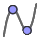
\includegraphics[width=0.0275\linewidth]{files/40px-Menu_view_algeb-122c1ab0ec365e77e9eae26ff7041249.png}

\textit{Graphing} in v prikazu 
\includegraphics[width=0.0275\linewidth]{files/16px-Menu_view_graph-07f951165e69080135ae4e0c7469a7db.png}

\textit{Graphics}, in sicer:


\includegraphics[width=0.7\linewidth]{files/344px-Toolbar-Graphi-8fcf80f609483dd4257ab538ddc900ac.png}

V nadelevanju opisujemo nekatere najpogosteje uporabljena orodja, celoten seznam orodij pa najdete v \href{https://geogebra.github.io/docs/manual/en/}{dokumentaciji Geogebre}.

Seveda, najlažji način za spoznavanje orodij je, da jih preizkusite sami v Geogebri!

\subsubsection{Vrstica za zamenjavo sloga}


\includegraphics[width=0.0275\linewidth]{files/40px-Stylingbar_icon-dbbb2f8b79b58bbc677f198035a192ed.png}

 \textit{Vrstica za zamenjavo sloga} (ang. \textit{Stylebar}) omogoča hitro spreminjanje grafičnih lastnosti izbranih objektov, kot so barva, debelina črte, slog črte in polnilo.
Ko izberete objekt v grafičnem oknu, se vrstica za zamenjavo sloga prikaže pod orodjarno in ponuja različne možnosti za prilagajanje videza izbranega objekta.
Možnosti so odvisne od vrste izbranega objekta, če ni objekta izbranega, vrstica za zamenjavo sloga prikaže možnosti sloga za pogled.

V vrstici za zamenjavo sloga se nahajajo samo osnovne možnosti, za dostop do naprednih možnosti sloga pa lahko kliknete na gumb 
\includegraphics[width=0.0225\linewidth]{files/32px-Settings.svg-c4703801fadb8667750afe6331c554d5.png}

 \textit{Nastavitve} (ang. \textit{Settings}), ki odpre pogovorno okno z več možnostmi za prilagajanje sloga izbranega objekta. Če ni izbranega objekta, gumb 
\includegraphics[width=0.0225\linewidth]{files/32px-Settings.svg-c4703801fadb8667750afe6331c554d5.png}

 \textit{Nastavitve} odpre pogovorno okno z možnostmi za prilagajanje sloga pogleda.

\subsubsection{Ukaze}

GeoGebra poleg grafičnih orodij ponuja tudi algebrske vnose in ukaze. Vsako orodje ima ustrezen ukaz, zato ga je mogoče uporabljati brez miške.

\begin{framed}
\textbf{Nasvet}\\
Dokumentacija za ukaze je v angleščini, zato je priporočljivo, da imate ukaze uporabite v angleščini.
Več o ukazih in njihovi uporabi najdete v \href{https://geogebra.github.io/docs/manual/en/}{dokumentaciji Geogebre}.
\end{framed}

\begin{framed}
\textbf{Opomba}\\
Vsaka orodoja ima svoj ukaz, obratno pa ne velja, obstajajo več ukazov kot orodij.
Večina uporabnikov Geogebra lahko brez težav dela z grafičnimi orodji, vendar moramo avtorji znati uporabljati ukaze. Tako bomo lahko delali hitreje in natančneje.
\end{framed}

Če hitro uporabimo ukaz, lahko ga vnesemo v \textit{Vrstico za vnos} (ang. \textit{Input Bar}), ki se običajno nahaja na dnu zaslona. Alternativno, lahko ukaze vnesemo tudi neposredno v grafično okno ali v 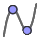
\includegraphics[width=0.0275\linewidth]{files/40px-Menu_view_algeb-122c1ab0ec365e77e9eae26ff7041249.png}

 \textit{Algebrsko okno} (ang. \textit{Algebra View}). Oboje lahko najdemo v meni ju 
\includegraphics[width=0.0275\linewidth]{files/32px-Menu-view.svg-287f1be47c2a7a168b1e84c64f1ec13c.png}

 \textit{Views}.

Naljažje način za spoznavanje ukazov je, da jih preizkusite sami v Geogebri!

\begin{framed}
\textbf{Nasvet}\\
Ko uporabite ukazi v Geogebri, je pomembno, da
upoštevate naslednje nasvete:

\begin{itemize}
\item Točke so definirane z velikimi črkami (npr. A, B, C), medtem ko so premice, daljice in krožnice definirane z malimi črkami (npr. a, b, c).
\item Pri vnosu koordinat točk uporabite oklepaje in vejice, npr. (2,3) za točko z $x$ koordinato 2 in $y$ koordinato 3.
\item Ukaz $v=(1,2)$ ne definira točke, ampak vektor z komponentama 1 in 2.
\item Uporabite  za samodejno dokončanje imen ukazov in objektov.
\item Uporabite  in  za navigacijo po zgodovini ukazov v vrstici za vnos.
\item Z gumbom 
\includegraphics[width=0.0225\linewidth]{files/24px-Menu-help.svg-0cd4dfd2862bbf9cf5b3df3fd837509b.png}

 \textit{Help} (sl. \textit{Pomoč}) (na desno od vrstice za vnos) lahko dostopate do dokumentacije Geogebre za ukaze.
\end{itemize}
\end{framed}

V Exercise~\ref{ex_GeogebraUkazi-1} ste se naučili

\begin{itemize}
\item Ustvariti geometrijske objekte z uporabo ukazov v vrstici za vnos.
\item Meriti kotov in dolžin in z uporabo orodje.
\item Prilagoditi besedilo z uporabo LaTeX formul.
\item Nastavitev \texttt{Starting point} za pozicioniranje besedila.
\end{itemize}


\bigskip
\centerline{\rule{13cm}{0.4pt}}
\bigskip

Geogebra nam omogoča vizualizacijo osnovnih geometrijskih konstrukcij in iskanje vzorcev v njih.
Na primer, pri konstrukciji v Exercise~\ref{ex_GeogebraUkazi-1} lahko opazimo, da je trikotnik $ABC$ vedno enakostraničen, ne samo za izbiro točko $A=(0,0)$ in $C=(4,0)$, ampak za katerokoli izbiro točk $A$ in $C$.
To lahko vidimo, če povlečemo točki $A$ in $C$ z orodjem 
\includegraphics[width=0.0225\linewidth]{files/32px-Mode_move.svg-b420ab97c3d398837a03b0709d9d93f2.png}

 \textit{Move}.
Opazimo da so dolžini stranici $AB$, $BC$ in $CA$ vedno enaki.
V Geogebri je to znano kot \textbf{test vlečenja} (ang. \textit{dragging test}), ki nam pomaga pri odkrivanju in dokazovanju geometrijskih lastnosti.

V prešnji konstrukciji smo uporabili \textbf{test vlečenja} (ang. \textit{dragging test}), ki nam pomaga pri odkrivanju in dokazovanju, da je trikotnik $ABC$ vedno enakostraničen.
S testom vlečenja lahko tudi vidimo, da so vsi koti v enakostraničnem trikotniku enaki in merijo $60^\circ$. To sledi iz dejstva, da je vsota notranjih kotov v trikotniku vedno $180^\circ$ in da so vsi trikotniki enakostranični.

\subsubsection{Algebrsko okno, proste točke vs. odvisne točke in kontrolni okvirček}

Vrstica za vnos ni edini način za interakcijo z Geogebro z uporabo ukazov.
Lahko uporabimo tudi 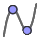
\includegraphics[width=0.0275\linewidth]{files/40px-Menu_view_algeb-122c1ab0ec365e77e9eae26ff7041249.png}

 \textit{Algebrsko okno} (ang. \textit{Algebra View}), ki prikazuje seznam vseh objektov v konstrukciji skupaj z njihovimi lastnostmi in vrednostmi.

Upoštevajte, da so točke \texttt{A} in \texttt{B} \textbf{proste točke} (ang. \textit{free points}), ker jih lahko premikamo kjerkoli v grafičnem oknu.
Vse ostale točke v konstrukciji so \textbf{odvisne točke} (ang. \textit{dependent points}), ker so določene z drugimi objekti v konstrukciji in se premikajo glede na spremembe teh objektov.
Proste točke so običajno modre barve, medtem ko so odvisne točke sive barve.
Seveda, to lahko spremenimo z uporabo vrstice za zamenjavo sloga ali v nastavitvah objekta, in torej barva ni zanesljiv indikator vrste točke.
V algebrskem oknu lahko vidimo katere objekte so proste in katere odvisne, saj so uporabimo gump \textit{Sort by} in torej \textit{Dependency} v vrstico za zamenjavo sloga algebrskega okna.


\bigskip
\centerline{\rule{13cm}{0.4pt}}
\bigskip

Kot smo videli, lahko uporabimo orodje 
\includegraphics[width=0.0275\linewidth]{files/32px-Mode_showhideob-4d2ce0e2e5642356a4a38fcbc8665f16.png}

 \textit{Show/Hide Object} za prikaz ali skrivanje objektov v grafičnem oknu.
To lahko storimo tudi v algebrskem oknu, kjer lahko kliknemo na krog levo od imena objekta za prikaz ali skrivanje objekta.
Poleg tega, lahko uporabimo tudi kontrolni okvirček (ang. \textit{checkbox}), ki ga lahko ustvarimo z orodjem 
\includegraphics[width=0.0275\linewidth]{files/32px-Mode_showcheckb-13e0b16b7961c33cdddba6a813116e81.png}

 \textit{Check Box} ali z ukazom \texttt{CheckBox()}.
Kontrolni okvirček vstavirte \textit{Check Box} v grafično okno in booleansko vrednost v algebrskem oknu.
Nato lahko uporabimo to vrednost za nadzor vidljivosti drugih objektov v konstrukciji.

\subsubsection{Izvoz konstrukcij kot slike.}

Lahko izvozimo naše konstrukcije iz Geogebre kot slike v različnih formatih, kot so \texttt{PNG}, \texttt{SVG} ali \texttt{PDF}.
Za izvoz konstrukcije kot slike, sledite tem korakom:

\begin{enumerate}
\item Pojdite na meni 
\includegraphics[width=0.0275\linewidth]{files/16px-Menu-file.svg-b74615e1101cba241695021ac4f1343d.png}

 \textit{File} in izberite 
\includegraphics[width=0.0275\linewidth]{files/24px-Menu-download.s-5fe900c8334923e022076eea13194034.png}

 \textit{Download as...}.
\item V pogovornem oknu izberite želeni format slike (npr. \texttt{.png}, \texttt{.svg} ali \texttt{.pdf}).
\item Posebni format je \texttt{PGF/TikZ}, ki omogoča izvoz konstrukcije kot kode, ki jo lahko uporabimo v LaTeX dokumentih.
\end{enumerate}

\subsubsection{Vaje}\label{07_geogebraUvod_vaje}

\begin{itemize}
\item Exercise~\ref{ex_GeogebraAccount}: Ustvarjanje računa Geogebra.
\item Exercise~\ref{ex_GeogebraTools}: Vaje za spoznavanje orodij Geogebre.
\item Exercise~\ref{ex_Stylebar}: Vaje za uporabo vrstice za zamenjavo sloga.
\item Exercise~\ref{ex_GeogebraUkazi-1}: Vaje za spoznavanje ukazov Geogebre.
\item Exercise~\ref{ex_dokazTrikotnik}: Vaje za dokazovanje lastnosti trikotnika z uporabo Geogebre.
\item Exercise~\ref{ex_TrikotnikKot}: Vaje za dokazovanje vsote notranjih kotov v trikotniku z uporabo Geogebre.
\item Exercise~\ref{ex_pentagram}: Vaje za ustvarjanje petkotnika in zvezde z uporabo Geogebre.
\item Exercise~\ref{ex_checkbox}: Vaje za uporabo kontrolnega okvirčka za nadzor vidljivosti objektov v Geogebri.
\end{itemize}